\documentclass[12pt]{article}
\usepackage{amsmath}
\usepackage{graphicx}
\usepackage{listings}
\usepackage{amsfonts}
\usepackage{amssymb}
\usepackage{hyperref}
\usepackage{tocloft}
\usepackage{multirow}

% \documentclass[tikz,border=10pt]{standalone}
\usepackage{tikz}
\usetikzlibrary{automata, positioning, arrows}

\usepackage[framed,autolinebreaks,useliterate]{mcode}

\title{Coursework 2 Answer}
\author{Junbiao Li - 209050796}
\date{\today}

\renewcommand{\cftsecleader}{\cftdotfill{\cftdotsep}}
% 对于 \section
\renewcommand{\cftsubsecleader}{\cftdotfill{\cftdotsep}}
% 对于 \subsection

\begin{document}

\maketitle
\tableofcontents

\clearpage
\section{Question a)}

\subsection{Question a) i)}

Recall that, for a European call option as
\[
    g\left(t, S_t\right)=S_t e^{-q(T-t)} \Phi\left(d_1\right)-K e^{-\rho(T-t)}
    \Phi\left(d_2\right)
\]
where
\[
    \begin{aligned}
         & d_1=\frac{\log \left(\frac{S_t}{K}\right)+\left(\rho-q+\frac{1}{2}
            \sigma^2\right)(T-t)}{\sigma \sqrt{T-t}}
        \\
         & d_2=d_1-\sigma \sqrt{T-t}
    \end{aligned}
\]

and we have \(S_0=5.35\), \(K=5.65\), \(\rho=5.4\% \), \(T=\frac{9}{12}=0.75\),
\(\sigma=0.3\). In addition, since the stock is non-dividend paying, we have
\(q=0\).

Hence, we have
\[
    \begin{aligned}
        d_1 & = \frac{\log
            \left(\frac{5.35}{5.65}\right)+\left(0.054+\frac{1}{2} \times
            0.3^2\right)
        \times 0.75}{0.3 \sqrt{0.75}} \\
            & =0.07578                \\
        d_2 & = d_1 - 0.3 \sqrt{0.75} \\
            & = -0.1840               \\
    \end{aligned}
\]
subtitute \(d_1\) and \(d_2\) into the formula, we have
\[
    \begin{aligned}
        g(0, S_0) & = S_0 \Phi(d_1) - K e^{-\rho T} \Phi(d_2)
        \\
                  & = 5.35 \Phi(0.07578) - 5.65 e^{-0.054 \times 0.75}
        \Phi(-0.1840)                                                  \\
                  & =0.5198
    \end{aligned}
\]

\subsection{Question a) ii)}

With Monte-Carlo simulation, we have European call option:
\[
    \begin{aligned}
        g\left(t, S_t\right) & =e^{-\rho(T-t)}
        \mathbb{E}\left[\left(S_T-K\right)_{+}
            \mid \mathcal{F}_t\right]
        \\
                             & \approx e^{-\rho(T-t)} \frac{1}{M}
        \sum_{i=1}^M\left(S_t e^{a(T-t)+\sigma z_i
                \sqrt{T-t}}-K\right)_{+}
    \end{aligned}
\]

Using MATLAB, which shown in appendix \ref{lst:a2}, we can have the following
solution

\begin{itemize}
    \item For M = 1000, the call option price is: 0.53721
    \item For M = 10000, the call option price is: 0.5059
    \item For M = 100000, the call option price is: 0.52095
    \item For M = 1000000, the call option price is: 0.51886
    \item For M = 10000000, the call option price is: 0.51948
    \item For M = 100000000, the call option price is: 0.51989
\end{itemize}

\subsection{Question a) iii)}

As we calculated in Question a) i), we expect the call option price to be
0.5198.

As the error is decreasing as M increases, we can see that the Monte-Carlo
simulation is converging to the true value, which is shown in Figure
\ref{fig:a_3}.

Hence we conclude that the as M increases, the Monte-Carlo simulation is more
accurate. In addition while M increases, the running time of the simulation
also increases.
\begin{figure}[htbp]
    \caption{Plot of the call option price against M}
    \label{fig:a_3}
    \centering
    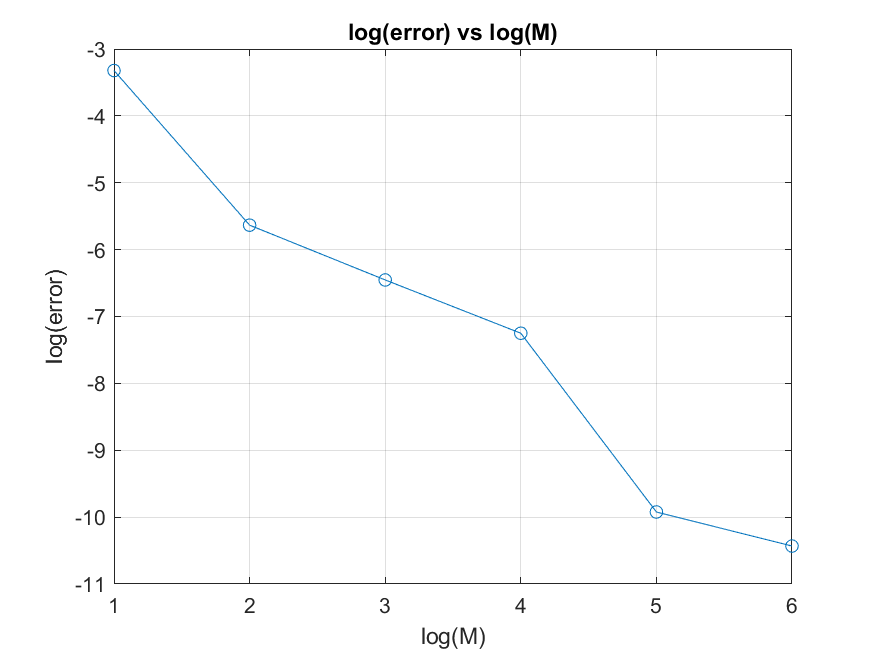
\includegraphics[width=0.8\textwidth]{imgs/a_2.png}
\end{figure}

\section{Question b)}

by adjusting the code in Question a) ii) to match exotic option payoff \(C=\max
\left(8 \cos \left(S_T\right)-5.65,0\right)\), which is shown in appendix
\ref{lst:b}, we have

\begin{itemize}
    \item For M = 1000, the exotic option price is: 0.50235
    \item For M = 10000, the exotic option price is: 0.49115
    \item For M = 100000, the exotic option price is: 0.48023
    \item For M = 1000000, the exotic option price is: 0.48059
    \item For M = 10000000, the exotic option price is: 0.48092
    \item For M = 100000000, the exotic option price is: 0.48067
\end{itemize}

\section{Question c)}

\subsection{Question c) i)}
We have \(S_0=5.35\), \(K=5.65\), \(\rho=5.4\% \), \(T=\frac{12}{12}=1\),
\(\sigma=0.3\).

Recall that,
\[
    \begin{aligned}
        \sigma_G & =\frac{\sigma}{\sqrt{3}}                           \\
                 & =0.1732                                            \\
        b        & =\frac{1}{2}\left(\rho-\frac{\sigma_G^2}{2}\right) \\
                 & =\frac{1}{2}\left(0.0054-\frac{0.1732^2}{2}\right) \\
                 & =0.0195                                            \\
        d_1      & =\frac{\log\left(\frac{S_t}{K}\right)+\left(b+\frac{\sigma_G^2}{2}\right)(T-t)}{\sigma_G\sqrt{T-t}}\\
                 & =-0.1158                                           \\
        d_2      & =d_1-\sigma_G \sqrt{T-t}                           \\
                 & =-0.1158-0.1732 \sqrt{1}                           \\
                 & =-0.2890
    \end{aligned}
\]
Hence, we can subtitute the values into the formula,
\[
    \begin{aligned}
        g\left(0, S_0\right) & =S_0 e^{(b-\rho)T}
        \Phi\left(d_1\right)-K e^{-\rho T} \Phi\left(d_2\right)                                   \\
                             & =5.35 \times e^{(0.0195-0.054) \times 1} \Phi(-0.1158)-5.65 \times
        e^{-0.054 \times 1} \Phi(-0.2890)                                                         \\
                             & =0.2782
    \end{aligned}
\]

\subsection{Question c) ii)}

For the Monte-Carlo simulation, we used a matrix sampling M points at a time.
Then do the calculation n times for simulating Asian call option. The code is
shown in appendix \ref{lst:c2},

Using MATLAB we have the following solution

\begin{itemize}
    \item For M = 1000, the asian option price is: 0.28874
    \item For M = 10000, the asian option price is: 0.2827
    \item For M = 100000, the asian option price is: 0.28446
    \item For M = 1000000, the asian option price is: 0.28123
    \item For M = 10000000, the asian option price is: 0.28159
\end{itemize}

\clearpage
\appendix
\section*{Appendix}
\addcontentsline{toc}{section}{Appendix}
\renewcommand{\thesubsection}{\Alph{subsection}}

\subsection{MATLAB Code}

\begin{lstlisting}[label=lst:a2,
    caption=Question a)ii)]
    S0 = 5.35; 
    K = 5.65; 
    r = 0.054; 
    T = 0.75; 
    sigma = 0.3; 
    
    Ms = [1000, 10000, 100000, 1000000, 10000000, 100000000];
    
    gt = 0.5198;
    
    for i = 1:length(Ms)
        M = Ms(i);
        callPrice = MonteCarloCallPrice(S0, K, r, T, sigma, M);
        disp(['For M = ', num2str(M), ', the call option price is: ', num2str(callPrice)]);
    end
    
    % plot error
    errors = zeros(length(Ms), 1);
    for i = 1:length(Ms)
        M = Ms(i);
        callPrice = MonteCarloCallPrice(S0, K, r, T, sigma, M);
        errors(i) = abs(callPrice - gt);
    end
    
    plot(1:length(Ms), log(errors), 'o-');
    xlabel('log(M)');
    ylabel('log(error)');
    title('log(error) vs log(M)');
    grid on;
    saveas(gcf, 'a_2.png');
    
    
    function callPrice = MonteCarloCallPrice(S0, K, r, T, sigma, M)
        % calculate a
        a = r - 0.5 * sigma^2;
        
        % init callValues
        callValues = zeros(M, 1);
        
        % simulate M times
        for i = 1:M
            % generate a random number from standard Brownian motion
            z = randn;
            
            % calculate ST
            ST = S0 * exp(a * T + sigma * z * sqrt(T));
            
            % calculate call value
            callValues(i) = max(ST - K, 0);
        end
        
        % calculate call price 
        callPrice = exp(-r * T) * mean(callValues);
    end
    
\end{lstlisting}

\begin{lstlisting}[label=lst:b,
    caption=Question b)]
    S0 = 5.35; 
    K = 5.65; 
    r = 0.054; 
    T = 0.75; 
    sigma = 0.3; 
    
    Ms = [1000, 10000, 100000, 1000000, 10000000, 100000000];
    
    gt = 0.5198;
    
    for i = 1:length(Ms)
        M = Ms(i);
        callPrice = MonteCarloCallPrice(S0, K, r, T, sigma, M);
        disp(['For M = ', num2str(M), ', the exotic option price is: ', num2str(callPrice)]);
    end
    
    function callPrice = MonteCarloCallPrice(S0, K, r, T, sigma, M)
        % calculate a
        a = r - 0.5 * sigma^2;
        
        % init callValues
        callValues = zeros(M, 1);
        
        % simulate M times
        for i = 1:M
            % generate a random number from standard Brownian motion.
            z = randn;
            
            % calculate ST
            ST = S0 * exp(a * T + sigma * z * sqrt(T));
            
            % calculate call value
            callValues(i) = max(8 * cos(ST) - 5.65, 0);
        end
        
        % calculate call price 
        callPrice = exp(-r * T) * mean(callValues);
    end
    

\end{lstlisting}

\begin{lstlisting}[label=lst:c2,
    caption=Question c)ii)]
    S0 = 5.35;  
    K = 5.65;   
    r = 0.054;  
    T = 1;      
    sigma = 0.3; 
    
    Ms = [1000, 10000, 100000, 1000000, 10000000];
    n = 100;
    
    for i = 1:length(Ms)
        M = Ms(i);
        asianOptionPrice = AsianCallOptionMonteCarlo(S0, K, r, T, sigma, M, n);
        disp(['For M = ', num2str(M), ', the asian option price is: ', num2str(asianOptionPrice)]);
    end
    
    function asianOptionPrice = AsianCallOptionMonteCarlo(S0, K, r, T, sigma, M, n)
        dt = T / n;  
    
        % generate n time points
        t = linspace(dt, T, n);  
    
        % generate standard Brownian motion.
        Z = randn(n, M) * sqrt(dt);
    
        % calculate all stock prices
        S = S0 * exp(cumsum((r - 0.5 * sigma^2) * dt + sigma * Z, 1));
    
        % calculate each path's geometric mean
        A_T = exp(mean(log(S), 1));
    
        % calculate call value
        callValues = max(A_T - K, 0);
    
        % calculate call price 
        asianOptionPrice = exp(-r * T) * mean(callValues);
    end
    

\end{lstlisting}

\end{document}